% 270 words
% Limit: 500 words
\section{Method}

\subsection{The data}

We crossmatched the \mct\ catalog of stellar rotation periods, measured from
\kepler\ light curves, with the \gaia\ DR2 catalog.
Reddening and extinction from dust was calculated for each star using the
Bayestar dust map implemented in the dustmaps {\it Python} package
\citep{green2018}.
We estimated effective temperatures from dereddened \Gaia\ \gcolor\ color,
using an 8th-order polynomial relation calibrated using .... stars
\racomment{ask Jason for details}.
\begin{equation}
    \mathrm{T_{eff}} = 8960 -4802C + 1931C^2 -2446C^3 + 2669C^4 - 1324C^5 +
    301C^6 - 26C^7,
% 8959.8112335205078, -4801.5566310882568, 1931.4756631851196,
%           -2445.9980716705322, 2669.0248055458069, -1324.0671020746231,
%           301.13205924630165, -25.923997443169355]
\end{equation}
where C is \gaia\ \gcolor.

\begin{figure}
  \caption{
A \gaia\ color magnitude diagram showing the \citet{mcquillan2014} sample with
    extinction-corrected magnitudes, colored by rotation period.
We excluded photometric binaries and subgiants from our analysis by removing
stars above the two dashed lines.
The rotation periods of binaries and subgiants do not follow a Skumanich-like
braking law.
The rotation period gradient across the main sequence is visible by eye in
    this figure: young, rapidly rotating stars are located below the old,
    slowly rotating stars.
}
  \centering
    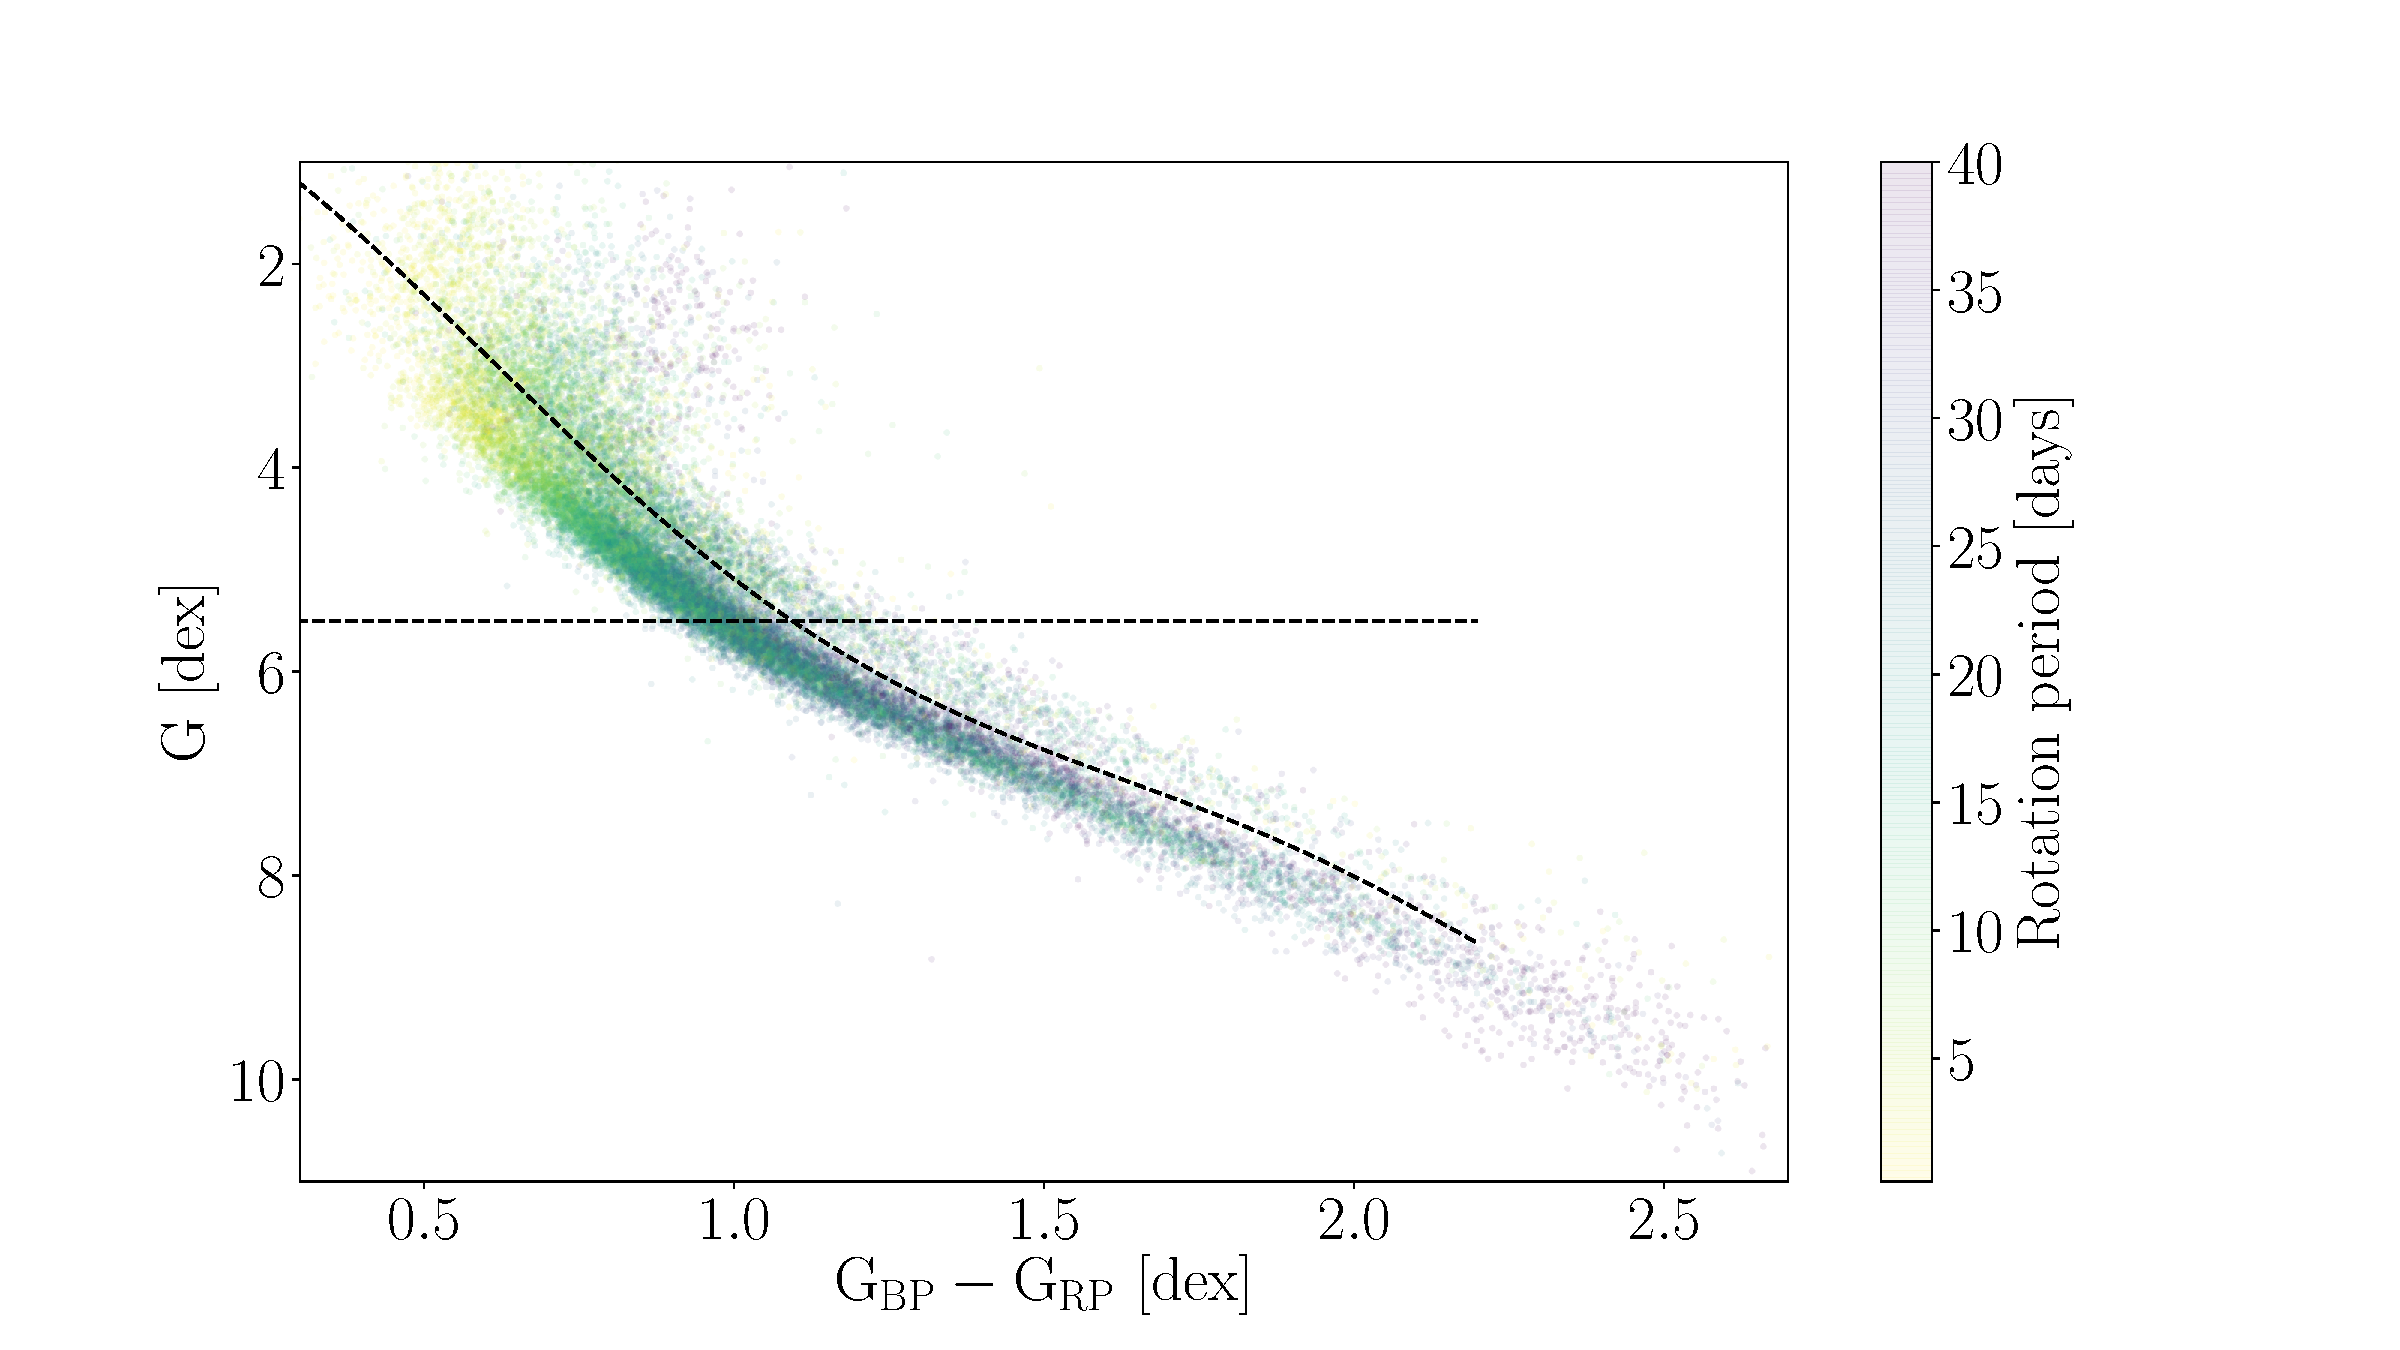
\includegraphics[width=1\textwidth]{CMD_cuts}
\label{fig:CMD_cuts}
\end{figure}
We removed visual binaries and subgiants from the sample as the
rotation-period evolution of these two types of stars is generally different
to that of single stars which more usually follow a Skumanich-like spin-down
law.
% Tidal and magnetic interactions between the two components of a binary system
% can influence the rotation periods of both stars, and the expanding envelopes
% of subgiants drive rapid spin-down through conservation of angular momentum.
We removed visual binaries and subgiants from the sample by applying cuts to
the color-magnitude diagram (CMD), shown in figure \ref{fig:CMD_cuts}.
We fit a 6th-order polynomial to the main sequence and raised it by 0.22 dex,
to approximate the division between single stars and visual binaries.
We eliminated visual binaries by removing all stars above this line from the
sample, and subgiants by removing stars brighter than 6th magnitude in \gaia\
G-band.

We removed stars with negative parallaxes and parallax signal-to-noise ratios
below 10 and a small number of stars fainter than 16th magnitude from the
sample.
We used the {\tt Pyia} \citep{price-whelan_2018} and {\tt astropy}
\citep{astropy2013, astropy2018} {\it Python} packages to calculate stellar
velocities.
{\tt Pyia} has built-in functionality for calculating velocity samples from
the full \gaia\ uncertainty covariance matrix via Monte Carlo sampling.
It therefore not only incorporates uncertainties on the \gaia\ positions
parallaxes and proper motions, it also accounts for the {\it covariance}
between these properties.
Finally, we removed stars with absolute \vb\ uncertainties greater than 1
\kms\ from the sample.

Gyrochronal ages were calculated using a polynomial gyrochronology relation
calibrated to Praesepe and the Sun \citep{angus2019}.
We used dereddened \gaia\ \gcolor\ color to calculate these ages.
Figure \ref{fig:period_teff} shows the \mct\ rotation period sample, separated
into three groups: stars above the gap in blue (classified as stars older than
1.1 Gyr), stars below the gap in orange (younger than 1.1 Gyr but older than
0.5 Gyr), and stars that are likely to be synchronized binaries (younger than
0.5 Gyr).
We used a gyrochronal isochrone (often called a gyrochrone) to separate these
groups of stars because the rotation period gap appears to fall on a
gyrochrone of 1.1 Gyr, and because the lower envelope of rotation periods is
also shaped like a gyrochrone at 0.5 Gyr.
This is probably because there is not a significant number of stars younger
than 500 Myr in the \kepler\ field.
Stars with short rotation periods, that seem younger than 500 Myr according to
the \citet{angus2019} gyrochronology relation are likely to be binaries.
Stars rotating more rapidly than 7 days were shown to be mostly synchronized
binaries \citep{citation}.
This is also borne out in the results section of this paper.
Although most rapid rotators are likely synchronized binaries (and therefore
not actually young -- just rotating rapidly because of tidal synchronization),
{\it some} of the rapid rotators probably {\it are} young and this could be an
extremely interesting group of stars from a scientific standpoint.

\begin{figure}
  \caption{
The rotation periods of stars in the \citet{mcquillan2014} sample vs.
effective temperature, with visual binaries and subgiants removed.
Blue circle points are non-photometric binary dwarfs, cooler than 4800 k, with
a rotation period and \gaia\ color indicating they are older than 1.1 gyr.
orange squares are stars that with rotation periods that fall just below the
gap: they have rotation-ages between 0.5 and 1.1 gyrs.
Green triangles are stars with rotation periods faster than the main envelope
of stars.
These are probably binaries whose rotation periods are synchronized to their
orbits and have been spun-up via tidal interactions.
}
  \centering
    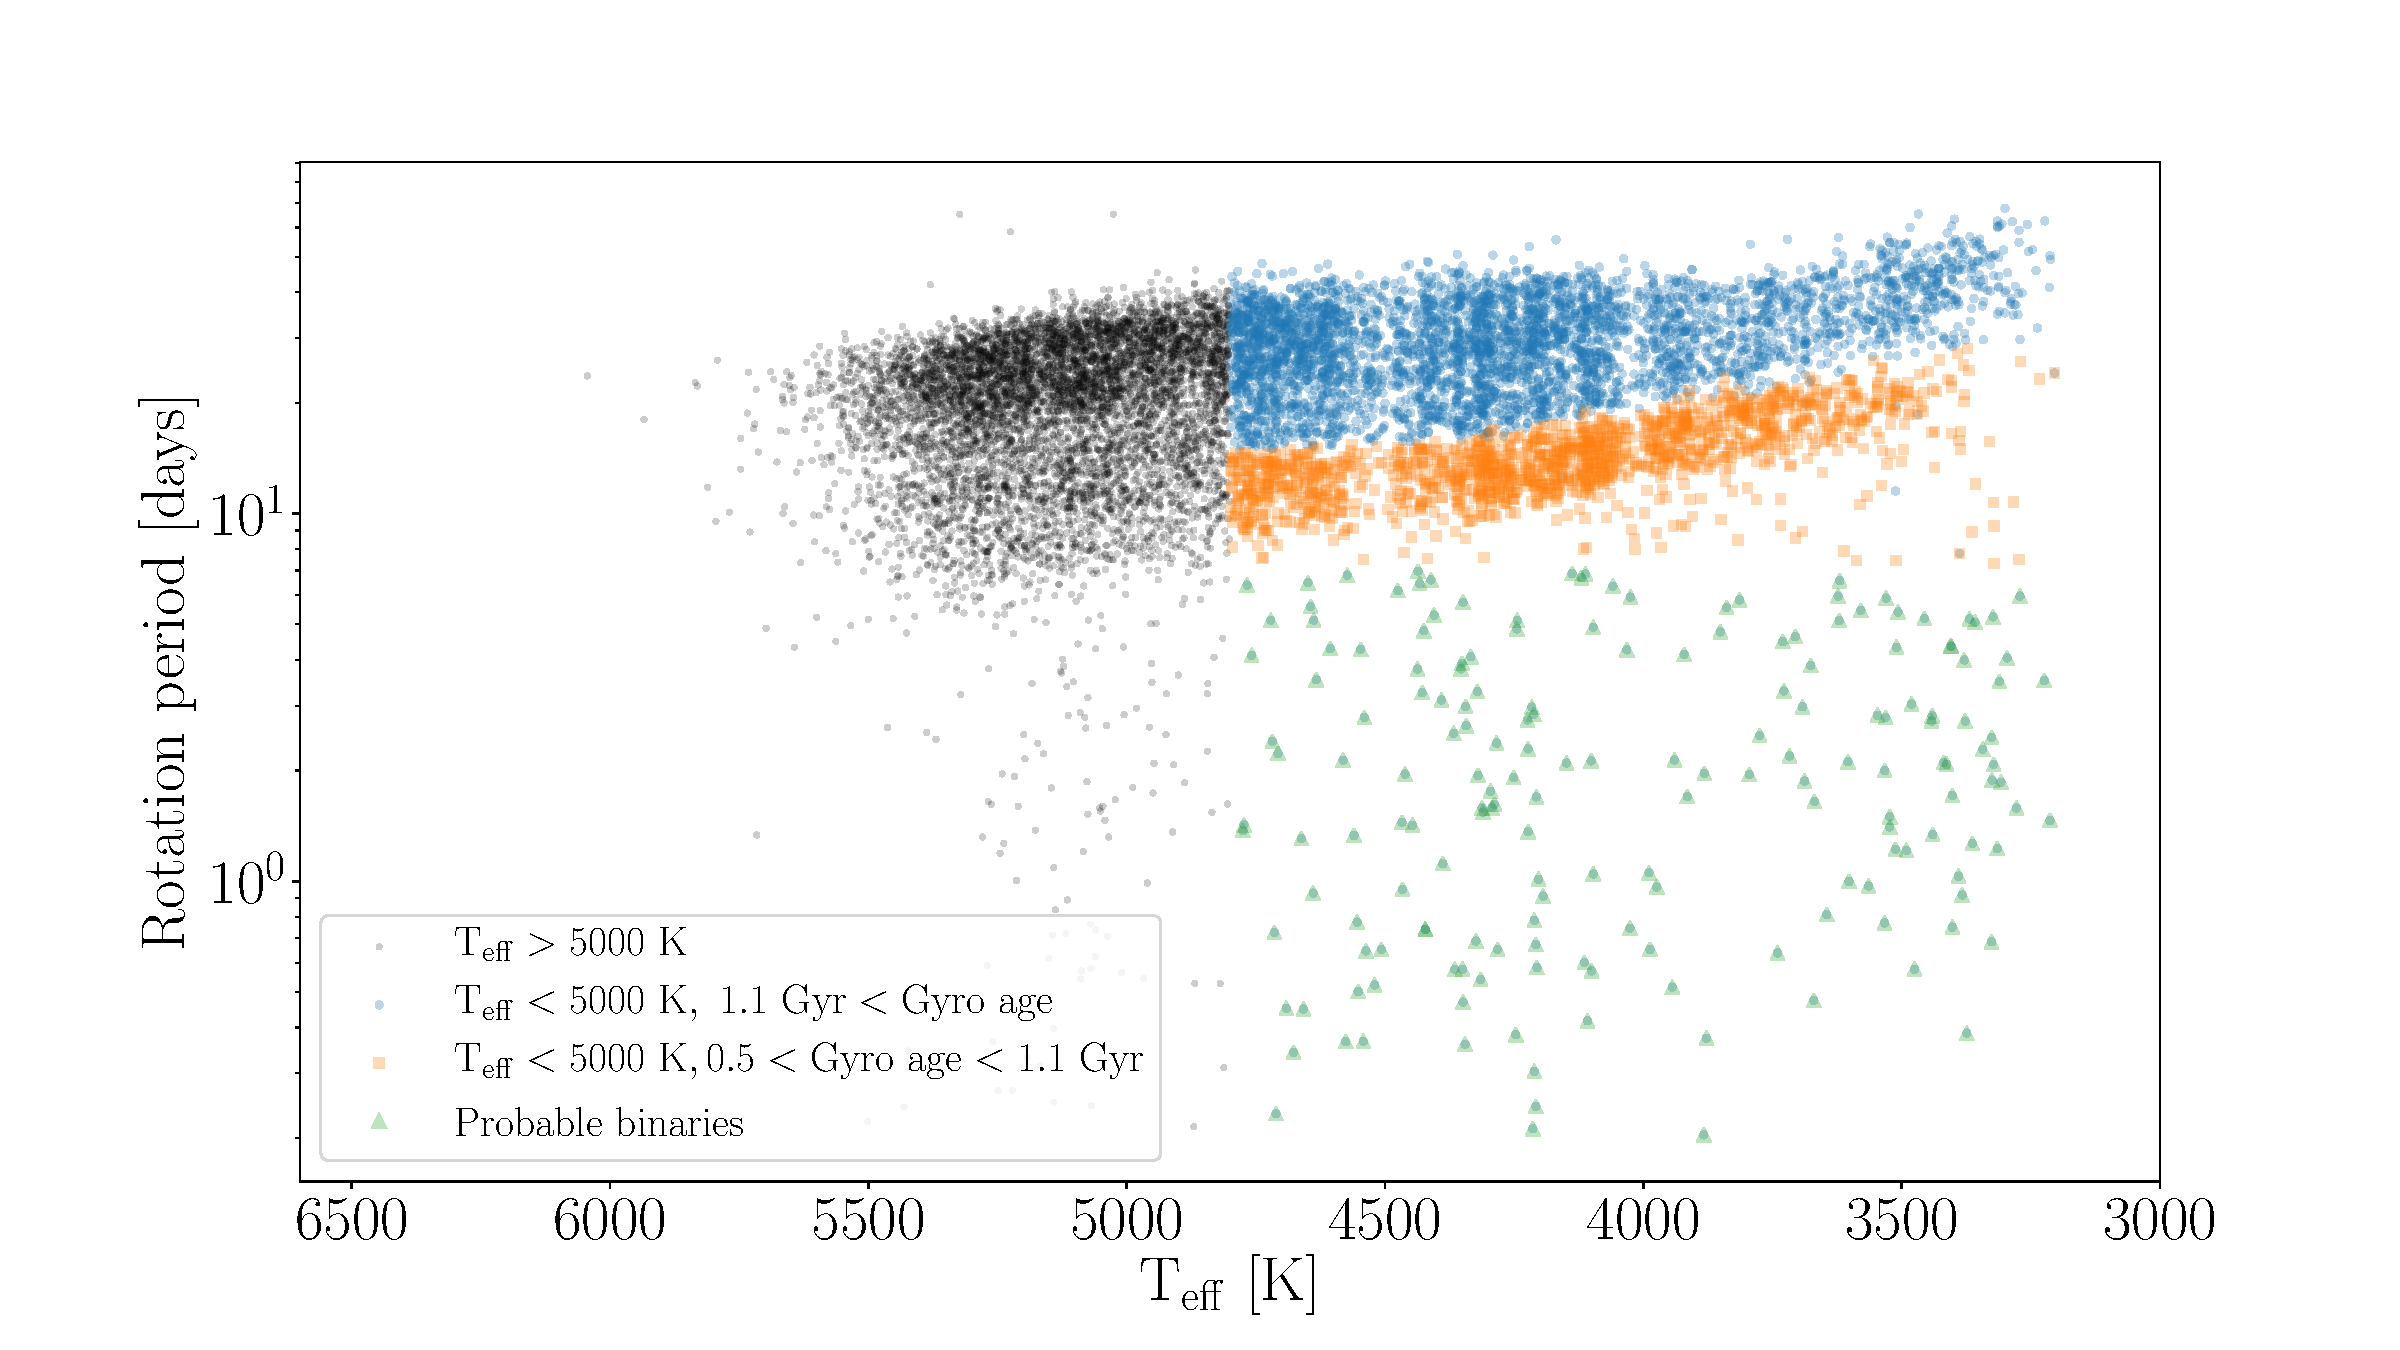
\includegraphics[width=1\textwidth]{period_teff}
\label{fig:period_teff}
\end{figure}
